\subsection{The Search and the Execution loop}%
\label{subsec:two_loops}
\todo[inline]{introduce search and execution loop}
\todo[inline]{Adding nodes always happens, in a backward search fashion}

\newpage
\newgeometry{left=1.1cm,bottom=0.1cm,top=1.9cm,headsep=0.1in,heightrounded}

\begin{figure}[H] 
\centering
\begin{tikzpicture}[node distance = 3cm]
    % Nodes
    \node [block, fill=yellow!50, line width=2pt, dashed] (first) {create start and target nodes};
    
    % legend
    \node[text width=2.8cm, yshift=1cm, right of=first, node distance=7cm, text centered, rounded corners, minimum height=1em, label={[name=lab, yshift=0.4cm, left]\textbf{Legend}}] (legend1) {\small Update KGraph};
    \node[rectangle, draw, left of=legend1, fill=green!50, rounded corners, minimum height=1em, minimum width=1cm, node distance=2cm] (legend1color) {};
    
    \node[text width=2.8cm, below of=legend1, text centered, minimum height=1em, node distance=0.7cm] (legend2) {\small Query KGraph};
    \node[rectangle, draw, left of=legend2, fill=red!40, rounded corners, minimum height=1em, minimum width=1cm, node distance=2cm] (legend2color) {};
   
    \node[text width=2.8cm, below of=legend2, text centered, minimum height=1em, node distance=0.7cm] (legend3) {\small Update C-Space};
\node[rectangle, draw, left of=legend3, fill=yellow!50, rounded corners, minimum height=1em, minimum width=1cm, node distance=2cm] (legend3color) {};
    
    \node[text width=2.8cm, below of=legend3, text centered, minimum height=1em, node distance=0.7cm] (legend4) {\small action in HGraph};
    \node[rectangle, draw, left of=legend4, rounded corners, minimum height=1em, minimum width=1cm, node distance=2cm, line width=2pt, dashed] (legend4color) {};
 
    \node[text width=2.8cm, below of=legend4, text centered, minimum height=1em, node distance=0.7cm] (legend5) {\small action in C-Space};
\node[rectangle, draw, left of=legend5, rounded corners, minimum height=1em, minimum width=1cm, node distance=2cm, line width=2pt] (legend5color) {};

    % nodes, Path exists 
    \node [decision, below of=first, node distance=2.6cm, line width=2pt] (path_existence) {Estimate Path Existence};
    \node [decision, left of=path_existence, node distance=4.5cm, line width=2pt, dashed] (subtasks) {Is there an unfinished Subtask};
    \node [block, above of=subtasks, node distance=2.7cm] (no_solution_found) {no solution found};
    
    % nodes, Knowledge available
    \node [decision, fill=red!40, below of=path_existence, node distance=3.2cm, inner sep=0.5mm] (know_avail) { Knowledge Available };
    \node [decision, fill=red!40, right of=know_avail, node distance=3.5cm, inner sep=0.5mm] (know_good) {Knowledge Usable};
    \node [decision, right of=know_good, node distance=3.5cm, inner sep=0.5mm] (movable) {Object Movable or Unknown};
    \node [block, left of=know_avail, node distance=3cm, line width=2pt, dashed] (impossible) {impossible task, abort subtask};
    
    % nodes, Generate new edge
    \node [decision, below of=know_avail, node distance=3.2cm, line width=2pt, inner sep=0.5mm, dashed] (goto_sys_iden) {Generate Random Edge};
    \node[block, right of=goto_sys_iden, node distance=3.5cm, line width=2pt, dashed] (no_trans_found) {No more edges available, abort subtask};
    
    
    % Motion/Manipulation planning 
    \node [decision, below of=goto_sys_iden, node distance=3.5cm] (single_multi) {Driving or Pushing?};

    \node [decision, line width=2pt, dashed, left of=single_multi, node distance=3.7cm] (model_avail_single) {Model available};
    \node [decision, line width=2pt, dashed, left of=single_multi, node distance=3.7cm] (model_avail_single) {Model available};
    \node [decision, line width=2pt, dashed, right of=single_multi, node distance=3.7cm] (model_avail_multi) {Model available};
    \node [block, line width=2pt, dashed, left of=model_avail_single, node distance=2.7cm] (sys_iden_single) {Add Sys. Iden. Node};
    \node [block, line width=2pt, dashed, right of=model_avail_multi, node distance=3cm] (sys_iden_multi) {Add Sys. Iden. Node};
    \node [block, line width=2pt, dashed, below of=single_multi, node distance=3cm] (move_object) {Add Node to Move Object};
    \node [block, line width=2pt, left of=move_object, node distance=3.7cm] (motion_planning) {Motion Planning};
    \node [block, line width=2pt, right of=move_object, minimum width=2.3cm, node distance=3.7cm] (manipulation_planning) {Manipulation Planning};
    \node [block, line width=2pt, dashed, minimum width=2.3cm, below of=move_object] (drive_to_object) {Add drive subtask to object};

    % nodes, Path to target
    \node [decision, below right of=drive_to_object, node distance=4.0cm, line width=2pt, dashed] (first_action) {First Action Planned};
    \node [decision, below left of=drive_to_object, node distance=3.5cm, line width=2pt, dashed] (global_path) {Path to Target}; 

    % \node [block, line width=2pt, dashed, minimum width=2.3cm] (drive_to_object) at ([xshift=0.1cm]$(move_object)!0.5!(global_path)$) {Add drive subtask to object};
    \node [decision, right of=first_action, diagonal fill={yellow!50}{green!50}, node distance=3cm] (execute) {Execute};
     
    % nodes, Target node reached 
    \node [decision, below of=global_path, node distance=3cm, line width=2pt, dashed] (target_node_reached) {Target Node Reached};
    \node [block, left of=target_node_reached, node distance=3cm] (end) {Task successfully executed};
    
    % Edges
    \path[line] ++(0,1.5) -- node[left]{task} (first);
    \path[line] (first) -- node[midway](to_path_exists){}(path_existence); 
    
    % edges, Path exists 
    \path[line] (path_existence) -- node[midway, above, left] {No path found} (impossible.north east);
    \path[line] (subtasks.north) --  node[left] {no} (no_solution_found);
    \path[line] (path_existence) -- node[xshift=0.08cm, yshift=0.35cm, right] {path found} (know_avail); 
    \path[line] (subtasks.east) -- node[above] {yes} (path_existence.west);
    
    % edges, Knowledge available
    \path[line] (know_avail) -- node[above] {yes} (know_good); 
    \path[line] (know_good) -- node[yshift=0.1cm, above] {no} (goto_sys_iden); 
    \path[line] (know_avail) -- node[left](toward_new_trans) {no} (goto_sys_iden); 
    \draw[->] (know_good.east) -- node[above] {yes} (movable.west);
    
    % \draw[-]  ([xshift=3.2mm]toward_new_trans.center) -| node[near start, above] {no} (know_good.south);
    \draw[-](impossible.west) -- +(-0.47,0); 
     
    \draw[->]  ([xshift=1.75cm, yshift=7.3cm]know_avail.center) --  node[at start, above] {action suggestions} ([xshift=1.75cm, yshift=1.75cm]know_avail.center) -- (know_avail.north east);
    \draw[->]  ([xshift=1.75cm, yshift=1.75cm]know_avail.center) -- (know_good.north west);
    \draw [draw=white,double distance=\pgflinewidth,ultra thick] (path_existence.east) -- +(2cm,0);
    
    % edges, Generate new edge
    \draw[-] (move_object.south) |- +(-8.2,-0.3);
    \draw [draw=white,double=black,double distance=\pgflinewidth,ultra thick] (motion_planning.south) -- +(0,-1cm);
    \draw[-stealth] (motion_planning.south)  -- ([yshift=-1cm]motion_planning.south) -| node[near start, above] {success} (global_path.north);
    \draw[-stealth] (manipulation_planning.south) |- node[near start, right] {success} (drive_to_object.east);
    \draw[-] (drive_to_object.west) -| (global_path.north);
    \draw[-] (motion_planning.west) -- node[above] {failure} +(-3.47,0);
    \draw[-] (manipulation_planning.east) -| node[near start, above] {failure} ([xshift=4.7cm,yshift=-0.6cm]no_trans_found.south) -- ([yshift=-0.6cm]no_trans_found.south);
    
    % edges, Single/Multi body
    \draw[-stealth] (single_multi.west) -- node[above] {driving} (model_avail_single);
    \draw[-stealth] (single_multi.east) -- node[above] {pushing} (model_avail_multi);
    \draw[-stealth] (model_avail_single.south) -- node[left] {yes} (motion_planning.north);
    \draw[-stealth] (model_avail_single.west) -- node[above] {no} (sys_iden_single);
    \draw[-stealth] (model_avail_multi.south) -- node[near start, left] {yes} (manipulation_planning.north);
    \draw[-stealth] (model_avail_multi.east) -- node[above] {no} (sys_iden_multi);
    \draw[-stealth] (motion_planning.east) -- node[above] {blockade} (move_object);
    \draw[-stealth] (manipulation_planning.west) -- node[above] {blockade} (move_object);
    \draw[-stealth] (goto_sys_iden) -- node[above] {failure} (no_trans_found);
    \draw[-] (sys_iden_single.north) --  ([yshift=1.07cm]sys_iden_single.north);
    \draw[-] (sys_iden_multi.north) |-  ([yshift=-0.6cm]no_trans_found.south);
    \draw[-] (no_trans_found.south) -- ++(0,-0.6cm) --([xshift=-8cm, yshift=-0.6cm]no_trans_found.south);
    \draw [draw=white,double=black,double distance=\pgflinewidth,ultra thick] (goto_sys_iden.south) -- node[at start, left] {success}(single_multi.north);
    \draw[-stealth] ([yshift=-0.5cm]goto_sys_iden) -- (single_multi.north);
    
    \draw[-] (movable.south) |- node[near start, left] {yes} ([xshift=-1.5cm, yshift=-1.4cm]movable.south) |- ([yshift=0.2cm]single_multi.north);
    \draw [draw=white,double distance=\pgflinewidth,ultra thick]  ([xshift=-1cm]movable.north) -- ([xshift=-8cm]movable.north);

    \draw[-] (movable.north) -- node[above]{no}([xshift=-8.23cm]movable.north);
    % HERE
    \draw [draw=white,double=black,double distance=\pgflinewidth,ultra thick] ([xshift=5.5cm,yshift=0.3cm]single_multi.north) -- ([xshift=5.5cm, yshift=2cm]single_multi.north);
    % \draw[-] (know_good.east) -| node[above]{yes} ([xshift=5.5cm, yshift=0.2cm]single_multi.north) -- ([yshift=0.2cm]single_multi.north);
    
    % edges, Path to target
    \path[line] (global_path) -- node[above] {yes} (first_action);
    \path[line] (first_action.east) -- node[above] {yes} (execute);
    \path[line] (global_path.west) -| node[left, below, near start] {no} ([xshift=-3cm, yshift=8.31cm]global_path.west) -|  (subtasks.south); 
   
    \draw[-stealth] (first_action.north east) -- node[near end, right] {no} ([xshift=1.7cm, yshift=0.39cm]first_action.north) |- ([yshift=-0.35cm]single_multi.south) -- (single_multi.south);
    \draw [draw=white,double=black,double distance=\pgflinewidth,ultra thick] (manipulation_planning.east) -- +(1cm,0);
    \draw [draw=white,double=black,double distance=\pgflinewidth,ultra thick] (manipulation_planning.north) -- +(0,1cm);
    
    \draw[-stealth] ([yshift=0.2cm, xshift=0.2cm]execute.south east) --  ([yshift=-0.8cm, xshift=1.2cm]execute.south east) -- node[at end, left] {robot input, action feedback} +(0,-2.7cm);
    
    \draw[stealth-] ([yshift=-0.2cm, xshift=-0.2cm]execute.south east) --  ([yshift=-1.2cm, xshift=0.8cm]execute.south east) -- node[left, at end] {sensor measurements} +(0, -1.8cm);
    
    \path[line] (execute.south) |- node[near start, left] {success} (target_node_reached.east);
    \draw[-stealth] (execute.east) -- node[above] {failure} ([xshift=1.5cm]execute.east) |- (path_existence.east);
    
    
    % edges, Target node reached 
    \path[line] (target_node_reached.north) -- node[left] {no} (global_path.south);
    \path[line] (target_node_reached.west) -- node[above] {yes} (end.east);
\end{tikzpicture}
\caption{Flowchart displaying the hypothesis graph's workflow.}
\label{tikz:flowchart_hgraph}% 
\end{figure}

\restoregeometry

\begin{figure}[H]
    \centering
    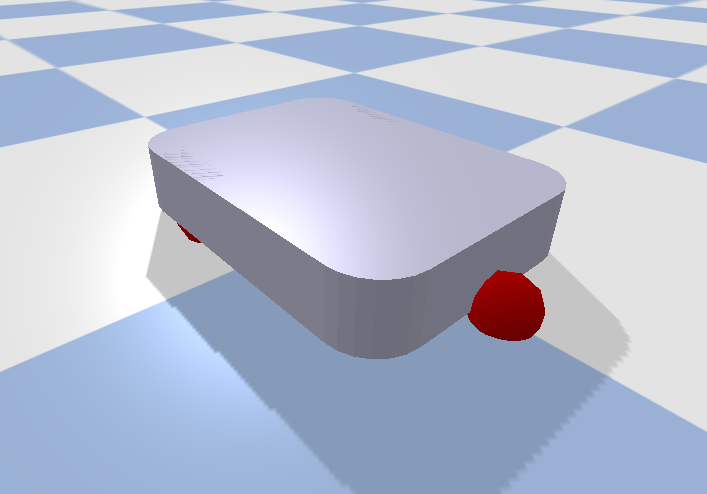
\includegraphics[width=5cm]{figures/boxer_robot.png}
    \caption{Pushing task through blocked corridor with the point robot, a green cube to push toward the target ghost state and a red blockade.}
    \label{fig:blocked_path_example_environment}
\end{figure}

\begin{figure}[H]
    \centering
    \begin{subfigure}{.5\textwidth}
    \centering
    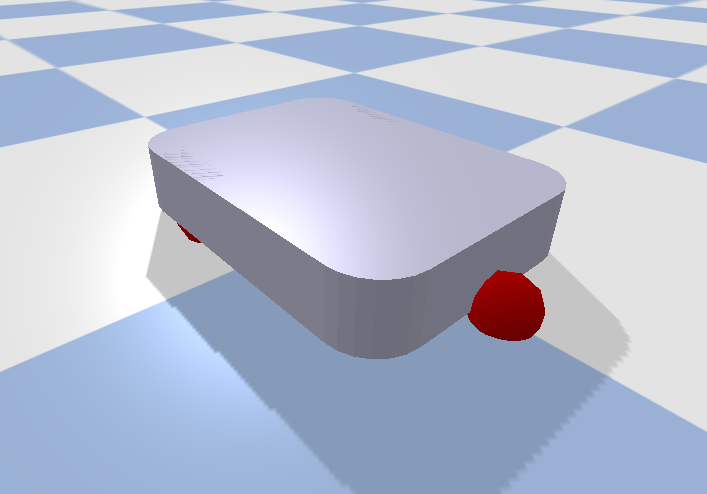
\includegraphics[width=0.8\textwidth]{figures/boxer_robot.png}
    \caption{todo}
    \label{subfig:todo}
    \end{subfigure}%

    \begin{subfigure}{.5\textwidth}
    \centering
    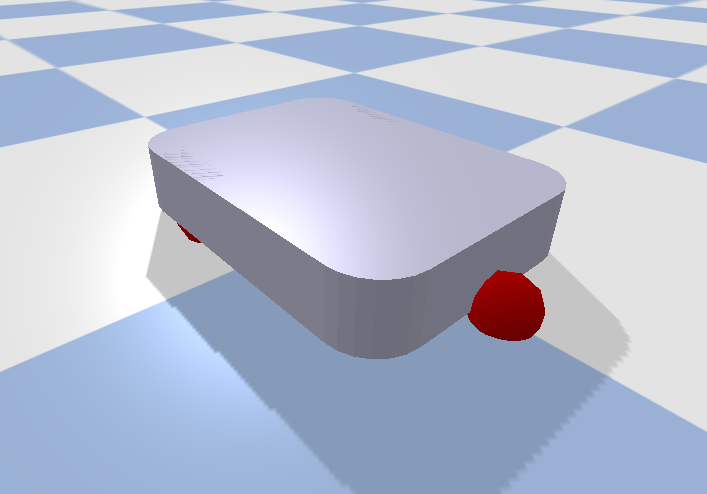
\includegraphics[width=0.8\textwidth]{figures/boxer_robot.png}
    \caption{todo}
    \label{subfig:B}
    \end{subfigure}
    \caption{todo}
    \label{subfig:blocked_path_hgraph_exmple}
\end{figure}

\todo[inline]{update the figure above here, Martijn did not like single/multi body, completely replace these terms.}
\todo[inline]{make the colors different, some which can be visualised with the airlab monitors.}

\todo[inline]{here are some example hgraph's required}

\todo[inline]{should I do an example Hgraph here? that requires target ghost positions. yes implement a }

As can be seen in \cref{tikz:flowchart_hgraph} there are some methods used which are still unexplained. Such as path non-existence, or motion planning. 
\todo[inline]{walk through the flowchart, what is actually happening here, It might be in your mind, but can the reader understand the flowchart without any additional context? clarify how edges are initialised, hypotheses are formed and how replanning occurs}
